\documentclass[10pt,twocolumn,letterpaper]{article}

\usepackage{cvpr}
\usepackage{times}
\usepackage{epsfig}
\usepackage{graphicx}
\usepackage{amsmath}
\usepackage{amssymb}

% Include other packages here, before hyperref.

% If you comment hyperref and then uncomment it, you should delete
% egpaper.aux before re-running latex.  (Or just hit 'q' on the first latex
% run, let it finish, and you should be clear).
\usepackage[breaklinks=true,bookmarks=false]{hyperref}

\cvprfinalcopy % *** Uncomment this line for the final submission

\def\cvprPaperID{****} % *** Enter the CVPR Paper ID here
\def\httilde{\mbox{\tt\raisebox{-.5ex}{\symbol{126}}}}

% Pages are numbered in submission Fmode, and unnumbered in camera-ready
%\ifcvprfinal\pagestyle{empty}\fi
\setcounter{page}{4321}
\begin{document}

%%%%%%%%% TITLE
\title{Sign Language Recognition}

\author{Daniel Gutowski\\
University of Warsaw\\
{\tt\small dg372207@students.mimuw.edu.pl}
% For a paper whose authors are all at the same institution,
% omit the following lines up until the closing ``}''.
% Additional authors and addresses can be added with ``\and'',
% just like the second author.
% To save space, use either the email address or home page, not both
\and
Jakub Kuklis\\
University of Warsaw\\
{\tt\small jk371125@students.mimuw.edu.pl}
\and
Filip Plata\\
University of Warsaw\\
{\tt\small fp371335@students.mimuw.edu.pl}
}

\maketitle
%\thispagestyle{empty}

%%%%%%%%% ABSTRACT
\begin{abstract}
	Sign languages are complex systems of hand gestures and body movements that are used for communcation, predominantly by deaf people and their interlocutors.
	In this report we present deep learning approaches we have used for static recognition of American Sign Language alphabet
	and for dynamic recognition of a semi-arbitrary set of gestures. For the static part, the training accuracy we have obtained is high,
	however the trained network does not recognize signs in our custom photographs. For the dynamic part, the training results are still unsatisfactory
	- the difficulty lies in understanding both the space and time context of the presented movements. 
\end{abstract}

%%%%%%%%% BODY TEXT
\section{Introduction}

The problem we are working on is recognition of gestures from standard RGB still images and clips.
Our main aim is to create a deep learning system that can be used to detect and classify signs from sign languages used around the world.
Such a system could be used to automatically generate transcriptions of texts conveyed with gestures,
or, after some extensions, to generate sign translations, when a proper human translation is not available.
One could also use that system to create a visual interface for detecting human intentions, like moving a virtual computer mouse.

We have chosen American Sign Language alphabet as the base for our experiments with static images, for a couple of reasons.
This language is widely studied in the deep learning community, which makes it easy to compare our results with the state-of-the-art models results.
There are a couple of large American Sign Alphabet datasets available on the internet.
ASL has also one of the largest communities of users, with approximately one million people using it as their main way of communication.
We have achieved a good test accuracy on ASL, however on photos we have taken, we could
recognize some groups of letters, like G and H or K, V and U. Signs for this letters are similar, which suggest our model has learned some aspects of sign language.

For the dynamic recognition, we have worked on a two of datasets, containing mostly hand gestures clips.
We have not obtained satisfactory results.
The challenge lies in the difficulty of understanding the space and time context of movements in clips presented to the neural network.


\section{Related work}

Results presented in the ~\cite{Google_signs} paper suggest that dividing sign recognition
into two problems - accurate hand position obtaining and then detecting signs -
is a promising method. Our approach uses that idea - for static
gestures, we first obtain a bounding box for a hand, and then proceed with
sign recognition. 

For dynamic signs, a lot of the work in the domain revolves around using
recurrent neural networks.
Another common trait is that most of the approaches consider images with more channels than just RGB, usually the depth parameter is also included.
We decided to use recurrent networks, but for regular RGB clips.
The article ~\cite{Jester_dynamic} influenced us in this respect, it used a sequence of 3D convolutions and LSTMs to obtain high accuracy for RGB videos. 


\section{Data}

\subsection{Static sign recognition}

We have used a dataset from Kaggle ~\cite{ASL_dataset}. It contains 90000 images of signs,
shown by one person. A lot of them look similar, but they are not syntetic. This dataset contains 200x200 RGB images. Data was
preprocessed with a neural network ~\cite{HandDetection} for hand detection and hand region
was rescaled to 64x64 resolution. This yielded an improvement
when using real word data, as only the hand is presented for the final classifier.
We have used augmentation - image shifts and rotations up to 5 degrees.

To allow us to pass any picture into the system we used approach described at \cite{Handtrack_dibia}.
It works on dataset which contains videos of hands movement around the frame. 
In this article author proposes network which can mark positions of hands basing solely on image.
We used network proposed in this paper as preprocessing to both our approaches.
However we did not obtain large improvements in dynamic hand sign recognition.

\subsection{Dynamic sign recognition}

We have used two different datasets.

We started by using the Boston dataset ~\cite{Boston_dynamic_signs, Boston_signs_article_1, Boston_signs_article_2}. 
It is a large collection of movies of people sitting in front of the camera and performing various signs. All of the images come in resolution of 480x640 pixels.
The dataset has metadata attached, which lists the frames in the video, when a given sign starts, and when it ends.
Its total compressed size is 4.6 GB, and uncompressed data didn't fit into 12GB of RAM.
Hence we needed a special loader implemented in Keras to load them from the disc.
We decided to move on to other datasets after encountering a couple of problems, mainly stemming from the scarcity of samples
- with only 4-5 samples per class, it was hard to make the network learn anything.
They also had a few issues from our perspective, for instance a complete answer to the problem lying in the left-top corner.
Furthermore, as the clips contain more than one sign and the breaks between them, a lot of frames do not carry much information.
Hence the need to extract distinct signs into separate file and masking of answer provided in corner.
In figure \ref{fig:boston_image} we present example data fed by us into network.

\begin{figure}
	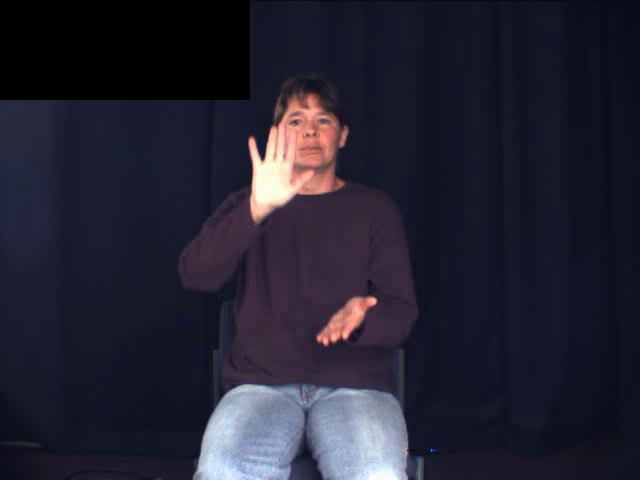
\includegraphics[width=\linewidth]{boston_dataset_gesture.jpg}
	\caption{Example data from Boston dataset}
	\label{fig:boston_image}
\end{figure}


Finally, we have used the twenty billion jester dataset ~\cite{Jester_dynamic}.
It contains clips of gestures used to perform different actions on the controlled system,
the clips have labels such as "swipe right" or "turn hand clockwise".
As there are 23GB of videos in the dataset and we were not able to load that all at once, we adapted the loader implemented for the first dataset.
Sample data can be seen in figure \ref{fig:jester_1}.

\begin{figure}
	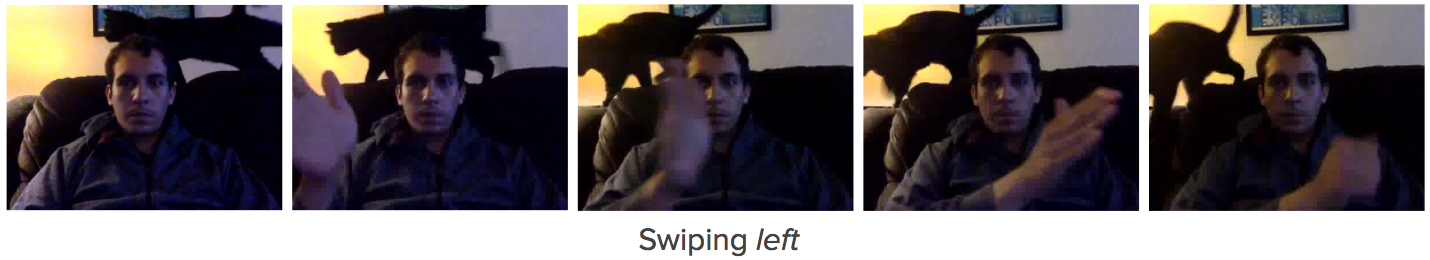
\includegraphics[width=\linewidth]{jester.png}
	\caption{Example data from Jester dataset}
	\label{fig:jester_1}
\end{figure}

\section{Methods}

\subsection{Static signs}

We have started with training a convolutional neural network based on various
examples we have seen during the course, without any preprocessing or augmentation.
Results on test dataset were up to about 96\% accuracy. The real word performance of
this approach on new images taken by us was extremely poor. The second approach
was to use hand detection first so that the sign classifier has more stable
performance. Along with augmentation, test accuracy dropped to 75\%, but
real world performance for some signs have improved. It became possible
to recognize G and H pair and also a group of signs which have two fingers spread
ot vertically.

The weak performance of the network might be a result of the dataset containing images of only one hand of the same person on virtually the same background.

\subsection{Dynamic signs}

We have tested a couple of neural networks architectures. Tree major ones were:

\begin{itemize}
	\item Applying CNN to consecutive images and inserting the result into a recurrent network,
	\item Training an auto-encoder to convert images into 2048 dimensional vectors, freeze its network and then feed it into a recurrent network,
	\item Applying 3-dimensional convolution layers and then feeding the result into recurrent network.
\end{itemize}

None of them proved to yield meaningful answers on any dataset.

\section{Experiments}

\subsection{Static signs}

Due to relatively poor performance on new signs, we did not conduct many experiments.
In figure \ref{fig:conf1} we have plotted confusion matrix and saw that similar signs like K and V are confused for
each other.

\begin{figure}
	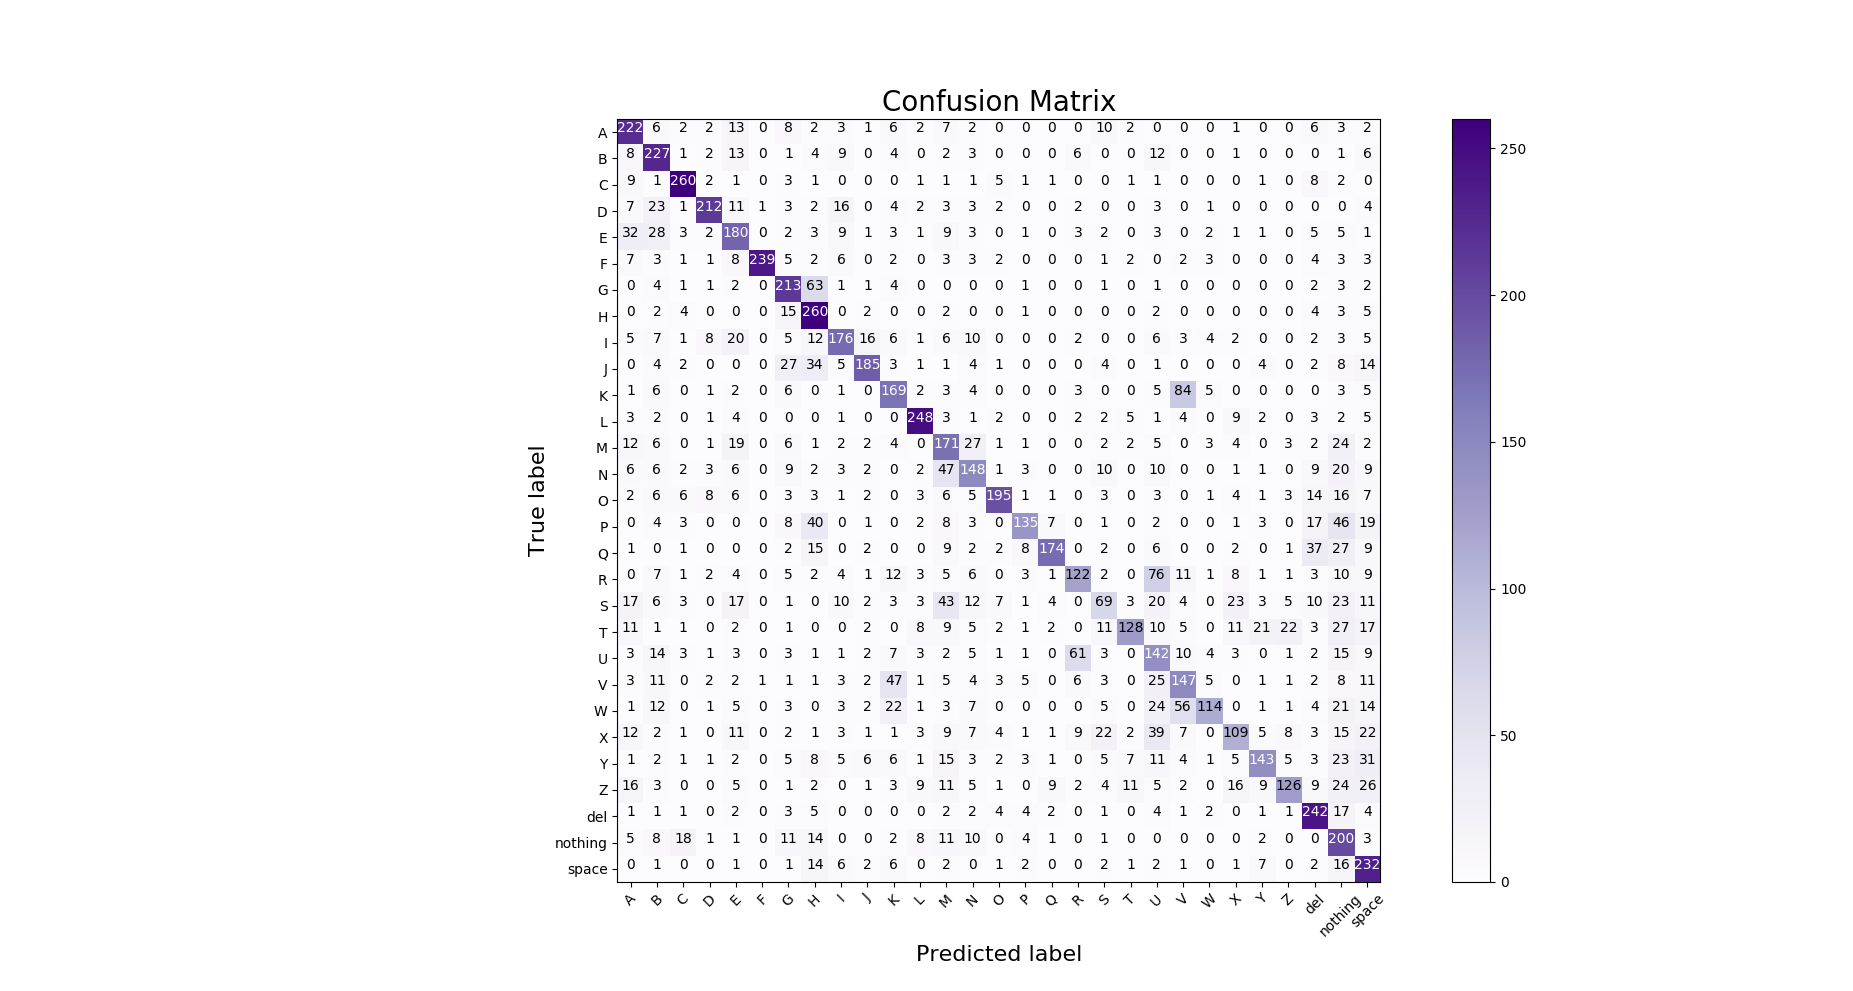
\includegraphics[width=\linewidth]{confusion_asl.png}
	\caption{Confusion matrix static ASL}
	\label{fig:conf1}
\end{figure}

Other similar signs are confused for each other, which is shows our model did learn
some key aspects. In figure \ref{fig:gesture1} we attach a sample new data for letter H - which performs well.
And in \ref{fig:gesture2} cropped image fed to static sign recognition network can be seen. 

\begin{figure}
	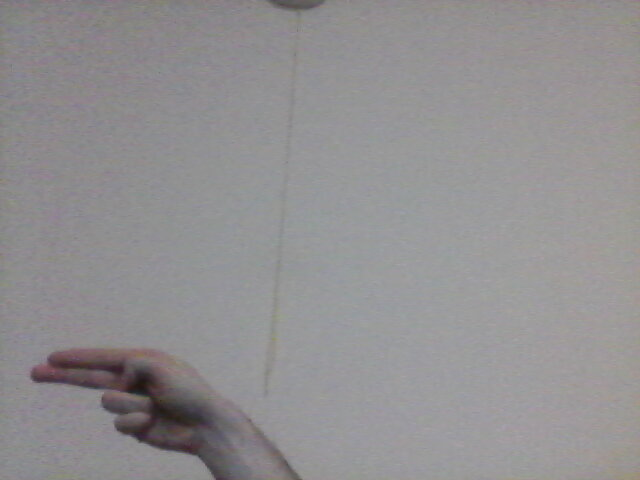
\includegraphics[width=\linewidth]{asl_h_1.jpg}
	\caption{Original image}
	\label{fig:gesture1}
	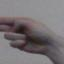
\includegraphics[width=\linewidth]{asl_h_1_focused.jpg}
	\caption{After hand-focus preprocessing}
	\label{fig:gesture2}
\end{figure}

\section{Conclusions}

One of the most important outcome is seeing for ourselves that splitting
a deep learning problem into pieces - just like any solid software - is
a valid approach, which not only makes sense, but also yields better results.
For the static part, a future extension would be to use a better full hand detection - producing
larger boxes, which would detect whole hand without cutting parts of fingers. 
Larger and richer datasets of various hands should also improve the
results on real word data.

We could see that learning dynamic signs is a very
hard problem. It requires connecting spatial information about the hands and arms position and the
timeframe of the movement. Thus, it might very useful to split the problem into two parts
- extracting information about hand/body postures, and only then feeding the recurrent neural network with processed data.

\section{Additional remarks}

While working in Keras, we have encountered a couple of obstacles that were hard to debug.
A memory leak bug in TimeDistributed wrapper set us back by a day, we needed to manually patch Keras
sources, since after fixing the bug it was not backported into version 2.0. 
Installing the newest version proved to be impossible due to differences in CUDA versions.
Also, in the default configuration, ~305MB of memory is allocated on every GPU, even if it never used.


{\small
\bibliographystyle{ieee}
\bibliography{egbib}
}

\end{document}
